
\chapter{The Database}

\section{Introduction to NoSQL Datbases}
The term NoSQL describes database systems that, unlike SQL databases, are not subject to the relational database model. The abbreviation NoSQL stands for "Not only SQL". The reasons why NoSQL databases have gained interest in recent years can be explained on the basis of two aspects: In contrast to relational databases, which present their data storage in table format, NoSQL databases benefit from different database models: document-oriented, key Value, graph and column databases.[Image] This wide range of different data models gives developers the benefit of being able to choose the model that best suits their application design. The resulting result is a minimization of the code to be developed for an application. In addition, NoSQL databases allow administrators to scale their data both on one machine and on hardware clusters, so data volumes can be expanded without an expensive investment in new servers.
\begin{figure}
	\centering
	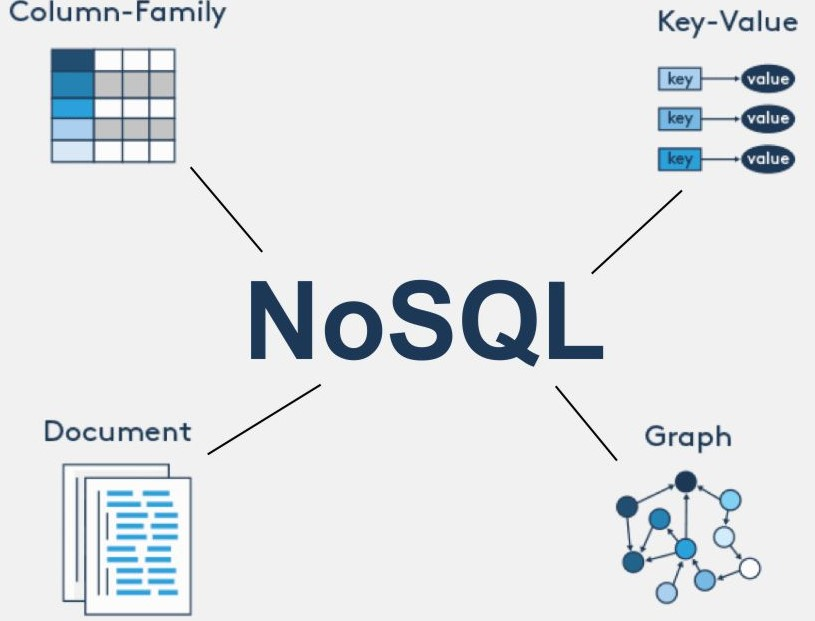
\includegraphics[scale=0.3]{nosql.jpg}
	\caption[NoSQL Data Models]{NoSQL Data Models}
\end{figure}
\section{Firestore}
Cloud Firestore, more often called Google Firestore, is a cloud-hosted NoSQL database option which enables developers to store and synchronize their data in realtime, meaning that data which just got added to the database and changes made on already existing data are instantly shown to the application users. Since Firestore is published by Google, it comes with peak reliablitly and great performance.  Firestore can easily be integrated in a Flutter Application with help of public packages and via the native SDKs. Something worth to mention is, that Firestore can be used with far more programming languages than Dart and is also compatible with REST and RPC APIs. Cloud Firestore caches data that your app is actively using, so the app can write, read, listen to, and query data even if the device is offline. When the device comes back online, Cloud Firestore synchronizes any local changes back to Cloud Firestore. To keep your data safe, firestore offers the opportunity to create security rules based on an individuals needs, this includes Identy and Access Management (IAM).

With Firestore in combination with Flutter one can retrieve data via the package cloud\_firestore and the StreamBuilder Widget provided by Flutter. The named package also allows the developer to make use of the authentication functionality provided by firestore, which makes it possible for a user to register and login in an application. A detailed example will be given later on, when adding and retrieving data becomes relevant in the diagnose-tracker-application. 

\section{Document Databases}
As mentioned in the introduction to NoSQL databases, there are several different databases which all rely on different data models. Firestore makes use of the document-based data format. This means, that data stored in the database is accessible via collections, which are filled with documents. For better understanding one can imagine a collection in Firestore as a table in relational Databases and a Document in Firestore equals a row in the relational schema. An example of that is shown in the figure x.x. Documents in Firestore store their data in a key-value-format which makes it possible for a developer to store different sort of documents in each collection. A quick view at an example makes this easier to understand: A developer wants to develop a restaurent-review application. For that he creates a collection named “restaurants” in firestore. Two of the three restaurants he now wants to add to the collection got a slogan with their brand which he wants to add to the documents, the other restaurant doesn’t have one. In a relational database he still would have to fill the “slogan” column with at least NULL-data or an empty String (or whatever datatype the column has). Firestore, or document-based databases in general, allow it, to just not add the slogan attribute to the third restaurant, which helps to only store relevant data to the database. It is important to keep in mind, that even if the third restaurant one day gets a slogan, the developer has the possibility to add that field to the document later on. Cloud Firestore also allows it to store subcollections or complex nested objects to documents. When wanting to recieve data from Firestore, one can simply 

\section{Designing a Data Structure}
Based on the information that emerged from the Requirements Engineering chapter, the class structures for the application can now be defined. Firestore supports the following datatypes:

\begin{itemize}
	\item String
	\item Number
	\item Boolean
	\item Map
	\item Array
	\item Null
	\item Timestamp
	\item Geopoint
	\item Reference
\end{itemize}

\subsection{Classes}
\subsubsection{User}
Users will be able to use the application without entering any personal details. As mentioned, Firestore offers an authentication and login functionality and with that the ability to sing in anonymously. When doing so Firestore will automaticly generate an anonymous account and add an user\_id and the timestamp of the account creation to the user-document in the database. One thing to mention about an anonymous account is, that the user will not be able to get his account back once he uninstalled or signed out of the application.
To fullfill the functional requirement [number], any user needs to be able to identify as a doctor. By doing so, the user account will be converted to a permanent account and the user, by then the doctor, is able to login, logout and uninstall the application without further consequences.
\subsubsection{Doctor}
When a user successfully verfied himself as a doctor, he gets access to all methods offered by the doctor class. The methods that come with this class are following:
\begin{itemize}
	\item \textbf{logout():} The doctor signs out of the application. That makes him a normal user and he has to login again.
	\item \textbf{editData(DataType pDataType):} The system shows the edit screen of the chosen either Symptoms, Causes, Diseases or Tips to the  
	
\end{itemize}
\section{Constructing Data Contexts}
\section{Inserting the Data into the Database}
\section{Firebase Redundancy}sc
\section{Connecting the Database with the Flutter Project}
